\documentclass[12pt]{article}
\usepackage{amsfonts}
\usepackage{graphicx}
\title{Thesis Proposal:  Chaos in Artificial Neural Networks}
\author{Ralph Bean\\
Department of Computer Science\\
Rochester Institute of Technology\\
\texttt{ralph.bean@gmail.com}}
\pagestyle{headings}
\begin{document}
\maketitle
\abstract{
Neural networks with chaotic baseline behavior are interesting for
their experimental bases in both biological relevancy and engineering
applicability.  In the engineering case, the literature still lacks a
robust study of the interrelationship between particular chaotic baseline
network dynamics and "online" or "driving" inputs.  We ask the question,
for a particular neural network with known chaotic baseline
behaviour, what periodic inputs of minimal magnitude have a
    stabilizing effect on network dynamics?  A genetic algorithm is
    developed for the task.  A systematic comparison of different
    genetic operators is carried out where each operator-combination is
    ranked by the optimality of solutions found.  The algorithm reaches
    acceptable results and finds input sequences with largest elements
    on the order of $10^{-3}$.  Lastly, an illustration of the complexity
    of the fitness space is produced by brute-force sampling period-2
    inputs and plotting a fitness map of their stabilizing effect on the
    network.
}
\vfill
\textbf{Thesis Committee}

\textbf{Adviser:}\hspace{14pt}Dr. Roger Gaborski

\textbf{Observer:}\hspace{7pt}Dr. Peter Anderson

\textbf{Reader:}\hspace{18pt}Thomas Borelli


\newpage
\setcounter{secnumdepth}{3}

\tableofcontents
\newpage

\section{Introduction}
The computational tasks of nonlinear classification and control are of high
importance to those interested in vision and acoustics.  The information
of interest in real world signals is most often embedded intrinsically in
their temporal structure.  Examples include distinguishing between and
producing the subtleties of human speech and predicting natural time series 
such as weather patterns and radioactive decay \cite{verstraeten, weigend}.

For many tasks, humans out-compete state-of-the-art computational techniques
hands-down in both accuracy and flexibility.

Consequently, techniques regarding recurrent neural networks
are of interest to computing research as a potential solution which could
harness the hard work already done for us computer scientists by the process
of biological evolution itself.

A large amount of theory has been developed with regard to feed-forward
neural networks from how to train them in both supervised and unsupervised
paradigms as well as why and how they work.  Things are not as nice when
we consider networks that have recurrent connections or feed-back connections.
Doya \cite{doya} 
provides an excellent description of the problems confronting gradient
descent for training recurrent networks.

The initial inspiration for this thesis came in 2001 from the work of
Jaeger \cite{jaeger_original}.
The Echo State Network (ESN) described there combined
a randomly generated recurrent network with a linear readout mechanism trained
to classify the state of the recurrent network.  It was observed that systems
that had randomly generated reservoir networks with dynamics at the 'edge of
chaos' performed better at temporal discrimination tasks.  This
thesis treats itself as a part of a process attempting to theoretically
explain the experimental success of Jaeger and others' work
\cite{maass_original}.

D. Verstraeten \cite{verstraeten} was the first
to use Lyapunov exponents as a measurement of chaos in the context of Jaeger's
work.  It must be stated that Verstraeten's application was built on a
misunderstanding of Lyapunov exponents.  In \cite{verstraeten},
only the first iteration
of the map defined by the network was considered in calculating Lyapunov
exponents.  Lyapunov exponents involve taking the limit of infinite
compositions of the map with itself which, for transcendental activation
functions like the hyperbolic tangent function most often considered for
artificial neural networks, is incalculable but can be approximated using
numeric methods \cite{sprott}.

The point of this thesis is to clarify notions of the edge of chaos
as they apply to artificial neural networks.  Sections 2 and 3 briefly describe
some background in artificial neural networks and dynamical systems theory.
Section 4 describes some examples of chaotic networks with no online input.
Section 5 relays some of the concepts and methods from control theory.
Section 6 details a genetic algorithm developed to investigate stabilizing
input streams for the network in section 4.2 along with some preliminary
results.  Section 7 reports results from the experiments devised in section 6.
Section 8 is a discussion of the results and section 9 contains concluding remarks.  All figures can be found in the appendix in section 10 starting on page 21.

\section{Artificial Neural Networks (ANNs)}
Artificial Neural Networks are a computational model of natural brains that
consist of a network of artificial neurons sometimes also called perceptrons.
These artificial neuron models activate more or less in response to
each other and a series of inputs as governed by a system of
equations \cite{jaeger_original, doya, dayan}.  They are perhaps best
contrasted with the Biological Neural Network or Spike/Pulsed Neural
Network computing models
which are more biologically realistic but more computationally expensive and
more theoretically unwieldy \cite{maass_book, fitzhugh, izhikevich_book}.

ANNs are defined by a choice of a weight matrix and activation function.
During simulation, the state of the $i$th neuron is calculated from the
weighted sum
of the state of all connected neurons in the previous timestep under
composition with the activation function.
\[ W= \left( \begin{array}{cccc}
             w_{1,1} & w_{1,2} & \cdots & w_{1,N} \\
                  w_{2,1} & w_{2,2} & \cdots & w_{2,N} \\
                       \vdots  & \vdots  & \ddots & \vdots \\
                            w_{N,1} & w_{N,2} & \cdots & w_{N,N} \end{array} \right)\]
$$x_{i,t+1} = f(\Sigma_{j=0}^{N} w_{i,j}x_{j,t})$$
$$\vec{x}_{t+1} = f(W \vec{x}_{t})$$


Although in some research, a variety of activation functions are chosen,
the two studied here will be
the hyperbolic tangent function
$$f(x) = tanh(x)$$
and the exponential sigmoidal function.
$$f(x) = (1 + e^{-\mu x})^{-1}$$
The hyperbolic tangent function has been proposed to best model the
'firing rate'
of more biologically plausible neural models.  Furthermore, the
universal approximation theorem states that a feed-forward ANN with the
hyperbolic tangent as the activation function and with a
sufficiently large hidden layer is able to approximate any continuous function
arbitrarily closely \cite{universal} which will be necessary for a
construction in section 4.  The exponential sigmoidal function is
relevant in its ability to elicit chaotic behavior in networks with simple
weight matrices

\section{Chaos in Nonlinear Systems}

A function $f : I \rightarrow I$ where $I \subset \mathbb{S}$ is said to be
chaotic \cite{hirsch} iff:
\begin{enumerate}
\item Periodic points of $f$ are dense in $I$;
\item $f$ is transitive on $I$;  that is, given any two subintervals $U_{1}$
and $U_{2}$ in $I$, there is a point $x_{0} \in U_{1}$ and an $n > 0$ such
that $f^{n}(x_{0}) \in U_{2}$;
\item $f$ has sensitive dependence in $i$; that is, there is a
\textit{sensitivity constant} $\beta$ such that, for any $x_{0} \in I$ and
any open interval $U$ about $x_{0}$, there is some seed $y_{0} \in U$ and
$n > 0$ such that
$$|f^{n}(x_{0}) - f^{n}(y_{0})| > \beta$$
\end{enumerate}

The set of periodic points of $f$ being dense in $I$ amounts to saying that
there are many such periodic points.  More formally, there exist points in $I$
that are surrounded by periodic points of $f$ with arbitrary closeness.

The second condition, the transitivity of $f$, amounts to a \textit{mixing}
requirement.  Points from $U_{1}$ at some time end up in $U_{2}$ and points
from $U_{2}$ at some time end up in $U_{1}$.  This follows from the above
property of the density of periodic points of $f$.

The third property, sensitive dependence on initial conditions alternatively
known as 'the butterfly effect', is the most popularly understood and the
more hotly contested aspect of chaos.  See \cite{history} for a thorough
treatment of the
confluence of Lorenz and non-mathematicians on broad cultural
misinterpretations of chaos theory.

A reasonable alternative to this condition involves characterizing
the \textit{rate} of separation of orbits by calculating
\textit{Lyapunov exponents} where the $k$th Lyapunov exponent, $h_{k}$, is defined as
$$h_{k} = \log \left( \lim \limits_{n \to \infty} (r_{k}^{n})^{\frac{1}{n}}\right)$$
Although we are most interested in the value of $h_{k}$
(is the rate of separation exponential or not?), introducing
the $k$th \textit{Lyapunov number} $L_{k}$ simplifies the equation
and is given by
$$L_{k} = e^{h_{k}} = \lim \limits_{n \to \infty} (r_{k}^{n})^{\frac{1}{n}}$$
For a trajectory through the state space, consider the effect had on the
points on a hypersphere of arbitrarily small radius centered on the
initial seed of the orbit.  Over the evolution of the system, this
hypersphere evolves into a hyperellipsoid.
The value of $r_{k}^{n}$ is the $k$th longest orthogonal axis of the
hyperellipsoid at the $n$th iterative application of
$f$ \cite{alligood, nikilov, verstraeten}.

In short, numerically approximating the Lyapunov exponents means
iterating the system into its future and measuring these axes \cite{sprott}.

\section{Construction of Chaotic Recurrent Networks}
By the universal approximation theorem, a three-layer feedforward artificial
neural network is able to approximate any continuous function arbitrarily
closely with a sufficiently large hidden layer \cite{universal}.
There are known chaotic maps.  For instance, the chaotic dynamics of the
logistic map $f_{4}$ are well
understood \cite{alligood, hirsch, devaney, sprott}.

\subsection{Training on the Logistic Map}

Consider a feed-forward network with topology $1 \rightarrow K \rightarrow 1$ 
that approximates $f_{4}$ with some error $\epsilon$.  Remove the single-neuron
output layer and replace all connections from the $K$ hidden neurons to that
neuron with identical connections back to the input layer.  It is clear that
the network is now recurrent and that its continued simulation computes the
iterative composition of the function the feed-forward network originally
modeled.  If the error $\epsilon$ between $f_{4}$ and the modeled function
is not too great, the iterated map now modeled by the network should be
qualitatively equivalent to the iteration of $f_{4}$ and orbits of the network
should exhibit chaotic motion.

The above was carried out by training a network to approximate $f_{4}$ with
standard back-propagation.  Experimental results are shown below in 
figures 1, 2, and 3.

The same process conceivably applies to other chaotic functions such as
$f(x) = \mu * x^{2} *(1-x)$ where $\mu=6.5$ and $f(x)=\mu * x^{3} * (1-x)$
where $\mu=8.1$.  Similar results were obtained but are not included in this
document.

\subsection{Other Known Chaotic Networks}
In \cite{sole} a network that exhibits chaotic behavior is described.  The
authors there document a 2-neuron network with weight matrix $W=$

\[ \left( \begin{array}{cc}
        -a & a \\
        -b & b \end{array} \right)\]

where $a=5$ and $b=25$ and activation
function $f_{\mu}(x) = (1 + e^{-\mu x})^{-1}$ (see figures 4 and 5).  
For different values of $\mu$,
this two-neuron network demonstrates many
different classes of dynamical phenomena including the so-called
period-doubling route to chaos as can be seen in figure 6.  Because of its
simplicity, it is the network used in experiments here.

\section{Control Theory}
A body of literature exists documenting theory and methods for the control
of chaotic systems.  Control of chaos falls into one of two complimentary
tasks:  stabilization and chaotization\cite{control_review}.
Bridging the two tasks are five main methods:  Open-loop control, Linear and
Nonlinear Control, Adaptive Control, Linearization of the Poincare Map (OGY),
Time-Delayed Feedback (Pyragas Method)\cite{control_review}.

The task of this thesis, stabilization of an unknown, chaotic, discrete-time 
neural network, rules
out the use of most of these documented approaches.  They are inappropriate
either because they apply only to continuous systems and not discrete, or
because they require fore-knowledge of the system to control, or because
they are strictly for the chaotization and not the stabilization of the
target system.

Stabilization of chaos using the OGY method has been documented
for discrete time neural networks \cite{yu}.
Application of OGY, however, relies on
the input signal or the controlling signal to have some knowledge of the
baseline dynamics of the system to be controlled and so is unsuitable for
the purposes here.

What remains applicable is Open-loop control (sometimes called vibrational
control).  Although there is a wealth of applications in the literature,
few are to discrete-time systems and of those, most are steeped in a
mathematical language unfamiliar to the author of this thesis.

The gist of open-loop or vibrational control is to find a finite-length set of
perturbations to the controlled system that elicit a periodic behavior in
it's otherwise aperiodic dynamics.  However, the \textit{amplitude} of the
perturbing impulses must be sufficiently small that the perturbations do
not simply override or 'wash out' the dynamics
of the system \cite{control_review}.


\section{Genetic Algorithm}
The above construction, as shown, can produce recurrent networks with
aperiodic motion under no input.  The spirit of neural network application,
however, is to perform some task on an input.  In the case of recurrent
networks as here, inputs with a temporal structure.

The question here asked is "does there exist a finite length input sequence
which, when presented under repetition, can stabilize an otherwise chaotic
neural network?"

The question is motivated by the reservoir computing application
\cite{jaeger_original, maass_original}.  There, for a readout
layer to converge on a decision, there must be some stabilization of the
reservoir.  Input sequences with no capacity for stabilization will
elicit seemingly random patterns from the network.  Sequences that
correspond to a stabilization of the reservoir will instead produce a sequence
of reservoir state vectors amongst which a readout layer can discriminate.

A genetic algorithm is developed to find such sequences for the network from
section 4.2.  Genetic algorithms are a technique designed to use
the principles of natural Darwinian evolution towards solving computational
problems.  Genetic algorithms (GAs) are distinguished by five components:  a
population of 'individuals' that are themselves potential solutions, a fitness
metric to rank how 'fit' each individual solution is or is not, a crossover
operator to breed and produce 'child solutions' from pairs of individuals,
a mutation operator to introduce new genetic material to the pool of
evolving solutions, and a selection operator to determine in what way
individuals are paired for crossover (reproduction) and in what way 
individuals are selected for discard (death).

\subsection{Genetic Operators}
In the application here, individuals in the population are
tuples consisting of a finite, variable length numeric sequence $S$ and an
amplitude coefficient $\alpha$.

Fitness of a $<S, \alpha>$ tuple is determined by
approximating the maximal Lyapunov exponent of the network
under perturbation by the sequence scaled
by an amplitude coefficient.  The maximal Lyapunov exponent is
measured as described in \cite{sprott}.  Loosely, it is a measure of 'how
stable' a system is.  A positive maximal Lyapunov exponent indicates exponential
expansion of orbits along at least one dimension of the system.  A negative
maximal Lyapunov exponent indicates exponential contraction along \textit{all}
dimensions.  For this genetic algorithm, minimal fitness
is 'better' fitness: exponential contraction of neighboring orbits indicates
stabilization.

Two major rounds of genetic experiments were run: preliminary and systematic.

\subsection{Preliminary Experiments (and results)}

In a first batch of experiments, the crossover operator is
single-point-crossover where two selected parents
have indices randomly selected from their sequences and two complimentary
children are created from the splicing together of each pair of subsequences.

The mutation operator alters a single element of a child sequence and
replaces it with a randomly chosen valid element.

Below are some preliminary results and observations that motivate the second
experiment.

\subsubsection{Binary Alphabet}
The first experiment run allowed for sequences to be composed only of elements
from the alphabet ${-1, 1}$ and for a fixed amplitude coefficient
$\alpha=0.00001$.  The choice of a value for $\alpha$ was arbitrary but was
chosen to be quite small as motivated by the discussion in section 5 on
vibrational control.

Two sub experiments were attempted with two different genetic selection methods.

Experiment 1 used the 'greedy' method where a child only replaces its parent if
its fitness is superior.  As can been seen from figure 7,
this apparently lead to premature convergence to a non-optimal solution.
The entire population converges to sequences with maximal Lyapunov exponents
of about 2.35 which is non-negative indicating a still chaotic network.

Experiment 2 did away with greedy selection and placed children in the
population without regard to their fitness.  From figure 8,
it appears this method effected an increase in diversity and developed
a sequence that could stabilize the network, a sequence with a negative
maximal Lyapunov exponent.

If the hero sequence did in fact stabilize the network, then we ought to see
a dramatic difference in the power spectral densities of the system with and
without the sequence present.  The PSD of the system running autonomously ought
to approximate $1/f$ while the PSD of the perturbed system ought to have one or more distinct peaks.  Experimental comparison did not align with this
hypothesis as shown in figure 9.  How can this be explained?

In both experiments 1 and 2 discussed so far, approximation of the maximal
Lyapunov exponent proceeded using a \textit{fixed seed}.  To see what effect
this may have had, a test of the exponent approximation function was conducted
on a sampling of initial seeds.  The result is shown in figure 10 and shows
that the algorithm stumbled on a numerical error in the approximation.
This was resolved by measuring the Lyapunov exponents at 25 different random
seeds and averaging the resultant values.

All further attempts to find a stabilizing input sequence using the above
method failed.

\subsubsection{Amplitude Coefficient}
In all of the above experiments, the amplitude coefficient $\alpha$ was
held at $0.00001$.  To investigate the effect this may have had, $\alpha$
was allowed to vary for simulation of the network under influence of the
hero from experiment 2.  Bifurcation diagram and Lyapunov exponents are
shown in figures 11 and 12, respectively.

Both figures indicate the appearance and disappearance of orderly and chaotic
windows as $\alpha$ varies away from $0$ in both directions.

This gives us reason to let $\alpha$ vary in genetic simulations and to
reformulate the task of the genetic algorithm as the combined minimization of
both the maximal Lyapunov exponent and the parameter $\alpha$.  We can see
from both figures 11 and 12 that with a sufficiently large value of $\alpha$,
the system can be forcibly stabilized, but ostensibly \textit{any} sequence
with a large enough $\alpha$ could accomplish such a task.  Again, the gist
is to apply as minimal an effect as possible while achieving the greatest
possible stabilization.

This has been implemented and first experiments show difficulty achieving a
values of $\alpha$ below $0.15$ which is unacceptably large.

The fitness function chosen was
$f(s, \alpha) = tanh(L(s)) + tanh(10(\alpha-0.12))$.  The function
was chosen to maximize the slope of the fitness surface around an area
that appeared to be a 'barrier' to further evolutionary progress using other
guesses at fitness functions.  A more systematic comparison of fitness
functions is in order.

\subsubsection{Real-valued Sequences}
A last set of preliminary experiments considered input sequences with
real-valued elements not restricted to a binary alphabet.  Between any two
distinct binary strings exists a continuum of real-valued strings along which
the bifurcation structure and Lyapunov surface varies smoothly.  Some of the
most optimal $\alpha$-sequence pairs found so far have $\alpha$ values
approaching $0.05$ and negative maximal Lyapunov exponents, apparently
indicating that more optimal solutions exist inbetween sequences with
strictly binary elements.

\subsection{Systematic Comparison}
In preliminary experiments, choices of fitness function and crossover and
selection operators were arbitrary.
Without a strong theoretical understanding of the problem, all three GA
components deserve a
systematic comparison of their effects on run-time behavior and best
solutions found.

In all, $4$ fitness functions, $10$ crossover operators, and $5$ selection
operators
are devised.  Of each combination, 4 trials were run.  Each trial was
terminated after $3500$ generations and took about $1.2$ hours to complete
which sums to about $40$ days of computing time.

\subsubsection{Crossover operators}
\begin{itemize}
\item "Random Single Point"  Subsequences of each parent sequence are selected by a random midpoint and exchanged to constitute complementary children (Figure 13).
\item "Fixed Single Point"  Subsequences of each parent sequence are selected by a fixed midpoint and exchanged to constitute complementary children (Figure 14).
\item "Gaussian Merge"  Gaussian merge crossover.  The value of each element of two parents are taken as standard deviations from a mean and used to construct a Gaussian distribution.  A random value is drawn from the distribution.  Its value is used as the value of the corresponding element in the first child's sequence and its complimentary value is used for the second child (Figure 15).
\item "Binary Random Single Point", and "Binary Fixed Single Point"  These two methods are identical to the random and fixed single point
methods described above except that sequence elements are first converted
to a binary representation and treated together as a then much longer sequence.
\item "DCT Random Single Point", "DCT Fixed Single Point", "DCT Gaussian Merge", "DCT Binary Random Single Point", "DCT Binary Fixed Single Point"  These five operators employ the same methods described above except that sequences are first passed through the discrete cosine transform and placed in the frequency domain before crossover is applied.  Children are then passed through the inverse discrete cosine transform to return them to the phase domain (Figure 16).
\end{itemize}
\subsubsection{Fitness functions}
\begin{itemize}
\item "Tanh Combination Metric" (Figure 17) $$f(<S,\alpha>) = tanh( L( <S, \alpha> ) ) + tanh( 10*(\alpha - 0.12) )$$
\item "Division Metric" (Figure 18) $$f(<S, \alpha>) = \frac{L( <S, \alpha> )}{\alpha}$$
\item "Addition Metric" (Figure 19) $$f(<S, \alpha>) = L( <S, \alpha> ) + \alpha$$
\item "Piecewise Metric" $$f( <S, \alpha>) = (L>0? L : \alpha)$$
\end{itemize}
\subsubsection{Selection operators}
\begin{itemize}
\item "Non Greedy Selection"  Four individuals are selected at random from the population.  The best two breed to produce children and the worst two are
replaced by the children (Figure 20).
\item "Greedy Selection"  Two individuals are selected at random for breeding.
Their children replace the worst two individuals in the population (Figure 21).
\item "Mutant Hero"  No crossover occurs.  The best individual in the population
is selected and two mutant children are produced.  They are inserted back in the
population in place of the worst two individuals.
\item "Greedy Mutant Hero"  A combination of the above selection methods.
Greedy selection is applied as above followed by an application of the mutant
hero method.
\item "Non Greedy Mutant Hero"  A combination of the above selection methods.
Non greedy selection is applied as above followed by an application of the
mutant hero method.
\end{itemize}
\subsection{Sampling the Problem Space}
Part of the motivation for such a robust comparison of genetic operators is
a genuine lack of theory about the relationship between driving inputs
network dynamics and without theory we cannot make intelligent choices.

The fitness landscape of the genetic algorithm formulated above is of quite
high dimension.  For input sequences of length $n$, a fitness landscape is
a $n$-dimensional manifold immersed in a $n+1$-dimensional space.  For $n > 2$
this cannot be visualized.  To give some idea of what solutions the GA is
searching through, a brute-force visualization of the Lyapunov surface is
carried out for the small toy-class of inputs of period 2.

Images are generated by mapping points on the plane $p=(x,y)$ to input
sequences $S_{x,y} = \lbrace x, y, x, y, x, .... \rbrace$.  A fitness map
is generated by measuring the Lyapunov number of each sequence $S_{x,y}$ and
plotting the Lyapunov number as an intensity value of the pixel associated
with $p=(x,y)$.

\section{Experimental Results}
The fitness map of the toy class of period-2 inputs is quite complex and appears in figures 22, 23, 24, and 25.  Its box-counting fractal dimension was measured at $1.914$.

The results of the systematic comparison are reported below.  Almost all
trials found solutions with negative (stabilizing) Lyapunov numbers.  Those
that did not were thrown out.

\vspace{20pt}

\begin{tabular}{|p{5cm}|p{2cm}|p{2cm}|}
\hline
\multicolumn{3}{|c|}{Table 1} \\
\multicolumn{3}{|c|}{By Fitness Function (200 experiments for each)} \\
\hline
Metric & Minimal $\alpha$ & Average $\alpha$ \\
\hline
\hline
Tanh Combination & 0.001078 & 0.199405 \\
\hline
Division  & 0.021248 & 0.259698 \\
\hline
Addition  & 0.045094 & 0.283053 \\
\hline
Piecewise & 0.021002 & 0.092758 \\
\hline
\end{tabular}

\vspace{20pt}

\begin{tabular}{|p{5cm}|p{2.0cm}|p{2.0cm}|}
\hline
\multicolumn{3}{|c|}{Table 2} \\
\multicolumn{3}{|c|}{By Selection Method (160 experiments for each)} \\
\hline
Selection Method & Minimal $\alpha$ & Average $\alpha$ \\
\hline
\hline
Non Greedy & 0.002770 & 0.276603 \\
\hline
Greedy & 0.001078 & 0.221014 \\
\hline
Greedy Mutant Hero & 0.021655 & 0.184394 \\
\hline
Non Greedy Mutant Hero & 0.009510 & 0.150492 \\
\hline
Mutant Hero & 0.015576 & 0.211140 \\
\hline
\end{tabular}

\vspace{20pt}

\begin{tabular}{|p{5cm}|p{2cm}|p{2cm}|}
\hline
\multicolumn{3}{|c|}{Table 3} \\
\multicolumn{3}{|c|}{By Crossover Operator (80 experiments for each)} \\
\hline
Crossover Operator & Minimal $\alpha$ & Average $\alpha$ \\
\hline
\hline
Random Single Point & 0.016584 & 0.173428 \\
\hline
Fixed Single Point & 0.024325 & 0.245391 \\
\hline
Gaussian Merge & 0.021655 & 0.222666 \\
\hline
Binary Random Single Point & 0.021248 & 0.184123 \\
\hline
Binary Random Fixed Point & 0.015576  & 0.213345 \\
\hline
DCT Random Single Point & 0.010714 & 0.174865 \\
\hline
DCT Fixed Single Point & 0.023137  & 0.253200 \\
\hline
DCT Gaussian Merge & 0.002770 & 0.184745 \\
\hline
DCT Binary Random Single Point & 0.001078 & 0.186835 \\
\hline
DCT Binary Fixed Single Point & 0.022892 & 0.248685 \\
\hline
\end{tabular}


\vspace{20pt}

Following are the 10 solutions found out of all 800 trials with the
overall smallest amplitude coefficients.

\vspace{10pt}

\begin{tabular}{|p{1.5cm}|p{3cm}|p{3cm}|p{3cm}|}
\hline
\multicolumn{4}{|c|}{Table 4} \\
\multicolumn{4}{|c|}{Top 10 Trials (by smallest $\alpha$)} \\
\hline
$\alpha$ & Fitness & Crossover & Selection \\
\hline
\hline
0.001078 & Tanh Combo & DCT Binary Random Point & Greedy \\
\hline
0.002770 & Tanh Combo & DCT Gaussian Merge & Non Greedy \\
\hline
0.009510 & Tanh Combo & DCT Binary Random Point & Non Greedy Mutant \\
\hline
0.010714 & Tanh Combo & DCT Random Point & Non Greedy Mutant \\
\hline
0.015576 & Tanh Combo & - - & Mutant Hero \\
\hline
0.016584 & Tanh Combo & Random Point & Non Greedy Mutant \\
\hline
0.018824 & Tanh Combo & DCT Random Point & Non Greedy Mutant \\
\hline
0.021002 & Piecewise &  - - & Mutant Hero \\
\hline
0.021248 & Division &  - - & Mutant Hero \\
\hline
0.021655 & Tanh Combo & Gaussian Merge & Greedy Mutant \\
\hline
\end{tabular}


\section{Discussion}
We can see from tables 1 and 4 that introduction of the hyperbolic tangent
fitness metric increased the probability of finding solutions with
extraordinarily small amplitude coefficients.  This metric was constructed
during preliminary experiments to address what appeared to be 'invisible
barriers' in the fitness space.  Populations tended to either clump at
small $\alpha$ but with $L > 0$ (unacceptable; still chaotic) or at
$\alpha > 0.12$ with $L < 0$ (acceptably stabilized but with unacceptably large
$\alpha$).  The metric was designed to maximize the slope of the fitness
surface along areas where populations were stagnating.  In retrospect, the
slope of the fitness surface really plays no role at all as a selection
pressure, but iso-fitness-curves do.  It appears to be the case that the
curves of equivalently-fit individuals through the fitness surface of the
'tanh combination metric' provide routes to small-$\alpha$ solutions not
otherwise accessible.

Take note also that while the piecewise metric did not develop many outstanding solutions, among fitness metrics it produced the best solutions on average.  It was
designed with much the same intent as the tanh combination metric (to maximize
the gradient in the direction most desired) but did not produce any optimal
solutions.

Results of the selection methods in Table 2 fail to demonstrate a clearly
superior method.  All five selection methods appear in the Top 10 table.
Greedy and Non Greedy standard selection eke ahead with the top best two
solutions found but comparison of their mean $\alpha$ values found with those
methods that take advantage of aggressive mutation demonstrates an inconsistency.  It is worth pointing out that the mutant hero method with \textit{no} crossover is outperformed by its peer methods.

The performance of crossover methods is a bit more difficult to take in simply
because so many were implemented.  All methods that involved the Fixed Single Point process performed poorly.  This is perhaps due to an imposed rigidity of
selective pressure that did not conform to the problem.  The Gaussian Merge method performed surprisingly poorly in isolation but stands out as one of the best methods when composed with the discrete cosine transformation.  As a group, methods that operated on binary representations of input strings did not perform well, the exception being the DCT Binary Random Single Point method.  The only logical grouping of operators that performed well, as a group, were methods that operated in the frequency domain, methods under composition with the discrete cosine transformation.

\section{Conclusion}

We can now answer positively to the central question posed in this thesis,
but the problems
approached here raise more questions.  We have found concretely that there
do exist finite length sequences of quite small amplitude that can,
under repetition as driving inputs,
stabilize an otherwise chaotic neural network.
Furthermore, subjective inspection of the brute-force sampling of the toy class 
indicates that arbitrarily small sequences are included in the set of
stabilizing inputs (Figure 26).

With regard to the application of genetic algorithms to stabilizing neural
networks, performing crossover in the frequency domain appears to have a
positive effect on algorithm convergence (Table 3).

Some open questions for future research:  does there exist a lower bound on
the amplitude coefficient of stabilizing sequences?  We have here found
sequences with amplitude on the order of $10^{-3}$ but yet smaller patterns
may exist.

While composition with discrete cosine transform in crossover
provided quite a boost to algorithm
performance, the choice of transform was somewhat arbitrary.
Does there exist a transform other than DCT that reduces the
complexity of the fitness space.  Future
research might be directed at the development of a genetic algorithm
that searches
through the space of transforms for ones that minimize the complexity of
the fractal in figure 22.

Other research might include consideration of networks that have been
shown to be useful in computational
tasks; this as opposed to the toy network studied here.  What
is the relationship between their usefulness in reservoir computing
techniques and their sets of stabilizing inputs?
Can we classify chaotic networks in terms of their
stabilizing sets?  Solutions to these questions are beyond
the scope of this document but in the author's estimation point the way toward
more fruitful applications of recurrent neural networks in the pursuit of
both scientific mastery and the unlocking of nature's mystery.

\begin{thebibliography}{widest-label}
\bibitem{alligood}
 K. Alligood, T. Sauer, J.A. Yorke
 \emph{Chaos:  An Introduction to Dynamical Systems},
 Springer-Verlag, 
 1997.
\bibitem{control_review}
 B.R. Andrievskii, A.L. Fradkov,
 \emph{Control of Chaos: Methods and Applications},
 Automation and Remote Control,
 vol. 64,
 pgs 673-713,
 2003.
\bibitem{arrowsmith}
 D. Arrowsmith and C.M. Place,
 \emph{An Introduction to Dynamical Systems},
 Cambridge University Press,
 1990.
\bibitem{universal}
 Balázs Csanád Csáji,
 \emph{Approximation with Artificial Neural Networks},
 Faculty of Sciences,
 Eötvös Loránd University,
 Hungary,
 2001.
\bibitem{clegg}
 J. Clegg, J. A. Walker, and J. F. Miller,
 \emph{A new crossover technique for Cartesian genetic programming},
 Proceedings of the 9th annual conference on Genetic and evolutionary computation,
 1580-1587,
 2007.
\bibitem{doya}
 K. Doya,
 \emph{Bifurcations in the Learning of Recurrent Neural Networks},
 Proceedings of the 1992 IEEE International Symposium on Circuits and Systems,
 2777-2780,
 1992.
\bibitem{devaney}
 R. L. Devaney,
 \emph{An Introduction to Chaotic Dynamical Systems},
 Westview Press,
 2003.
\bibitem{weigend}
 A. Weigend and N. Gershenfeld,
 \emph{Time Series Prediction.  Forecasting the Future and Understanding the Past},
 Addison-Wesley,
 1994.
\bibitem{history}
 D. Aubin and A. Dahan Dalmedico,
 \emph{Writing the History of Dynamical Systems and Chaos:  Longue Dur\'ee and Revolution, Disciplines, and Cultures},
 Historia Mathematica,
 vol. 29,
 pgs 273-339,
 2002.
\bibitem{dayan}
 P. Dayan and L. F. Abbott,
 \emph{Theoretical Neuroscience:  Computational and Mathematical Modeling of Neural Systems},
 The MIT Press,
 2001.
\bibitem{fitzhugh}
 C. Rocsoreanu, A. Georgescu, and N. Giurgiteanu,
 \emph{The Fitzhugh-nagumo model:  Bifurcations and Dynamics},
 Kluwer,
 2000.
\bibitem{hirsch}
 M. W. Hirsch, S. Smale, R. L. Devaney,
 \emph{Differential Equations, Dynamical System, and an Introduction to Chaos},
 Elsevier,
 2004.
\bibitem{izhikevich_book}
 E. Izhikevich,
 \emph{Dynamical Systems in Neuroscience:  The Geometry of Excitability and Bursting},
 The MIT Press,
 2007.
\bibitem{maass_what_makes}
 R. Legenstein and W. Maass,
 \emph{What makes a dynamical system computationally powerful?}
 Haykin, Principe, Sejnowski, and McWhirter:
 New Directions in Statistical Signal Processing:  From Systems to Brain
 2005.
\bibitem{maass_metaphor}
 T. Natschl\"ager, W. Maass, H. Markram,
 \emph{The "Liquid Computer":  A Novel Strategy for Real-Time Computing on Time Series}
  Special Issue on Foundations of Information Processing of TELEMATIK, 
  vol. 8, 
  num. 1, 
  p. 39-43,
  2002 
\bibitem{maass_book}
 W. Maass and C. M. Bishop,
 \emph{Pulsed Neural Networks},
 The MIT Press,
 1999.
\bibitem{maass_original}
 W. Maass, T. Natschl\"ager, and H. Markram,
 \emph{A Model for Real-Time Computation in Generic Neural Microcircuits},
 Proc. of NIPS 2002, 
 Advances in Neural Information Processing Systems, 
 volume 15, 
 pages 229-236. 
 MIT Press, 
 2003.

\bibitem{nikilov}
 S. Nikolov, and B. Bozhkov,
 \emph{Bifurcations and chaotic behavior on the Lanford system},
 Chaos, Solitons and Fractals
 vol. 21,
 pgs 803-808,
 2004.

\bibitem{norvig}
 S. Russell and P. Norvig,
 \emph{Artificial Intelligence: A Modern Approach},
 Prentice Hall,
 1995.

\bibitem{sole}
 R.V. Sole, L. Menendez, D.L. Prida,
 \emph{Controlling Chaos in Discrete Neural Networks},
 Phys Lett A,
 vol. 199,
 pgs 65-69,
 1995.

\bibitem{sprott}
 J. C. Sprott,
 \emph{Chaos and Time Series Analysis},
 Oxford University Press,
 2003.
\bibitem{jaeger_original}
  H. Jaeger,
  \emph{The "echo state" approach to analysing and training recurrent neural networks}.
  GMD Report 148, 
  GMD - German National Research Institute for Computer Science,
  2001.
\bibitem{verstraeten}
 D. Verstraeten, B. Scharuwen, M. D'Haene, D. Stroobandt,
 \emph{An experimental unification of reservoir computing methods},
 Neural Networks,
 vol. 20,
 pgs 391-403,
 2007.
\bibitem{yu}
 H. Yu, Y. Liu, J. Peng,
 \emph{Control of chaotic neural networks based on contraction mappings},
 Chaos, Solitons, and Fractals,
 vol. 22,
 pgs 787-792,
 2004.

\end{thebibliography}
\newpage
\section{Appendix of Figures}
\begin{figure}[htb]
\begin{center}
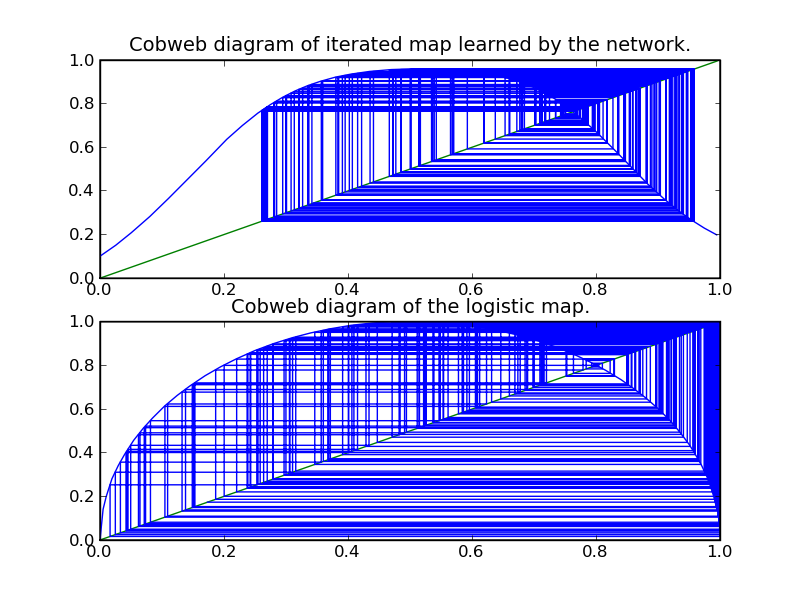
\includegraphics[height=2.5in,width=4.5in]{images/cobweb_1.png}
\caption{Cobweb diagrams are one way of visualizing the dynamics of iterated one-dimensional maps.  To generate the above images, a random seed between 0 and 1 was chosen.  The orbit was iterated 2000 times and only the last 200 iterations are plotted to ensure no stabilization from a seed chosen too far from the potentially strange attractor.}
\end{center}
\end{figure}
\begin{figure}[htb]
\begin{center}
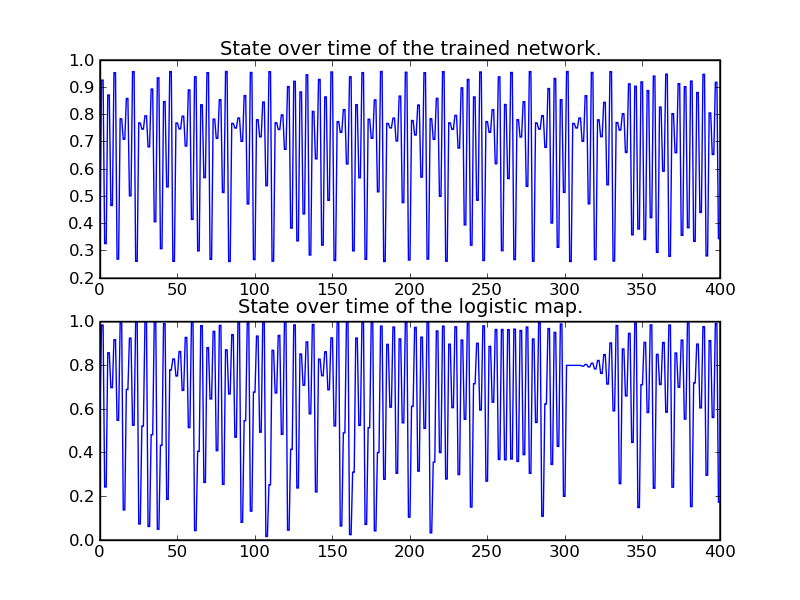
\includegraphics[height=2.5in,width=4.5in]{images/orbit_1.png}
\caption{Plot of the same orbits shown in the cobweb diagrams but against the timestep.}
\end{center}
\end{figure}


\begin{figure}[htb]
\begin{center}
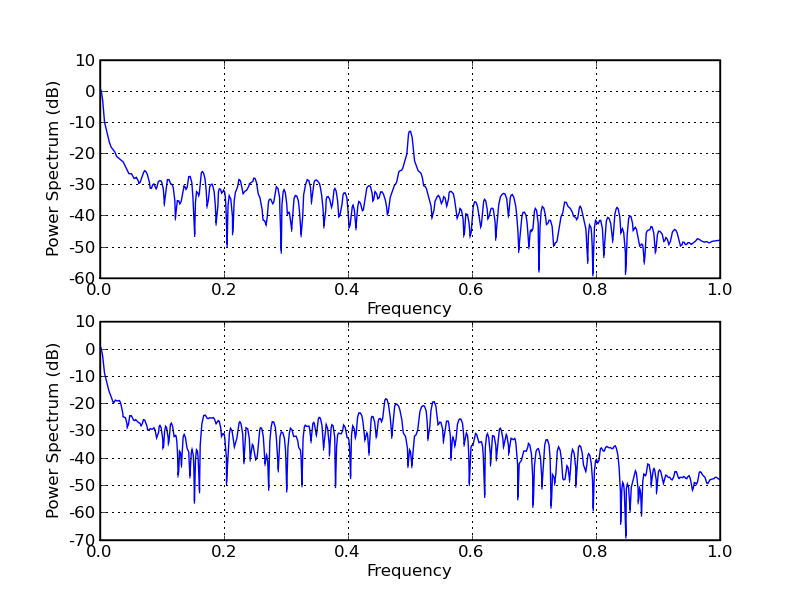
\includegraphics[height=2.5in,width=4.5in]{images/psd_1.png}
\caption{Power spectral density functions of the network and its target map.  In each case, the logarithm of the psd is plotted.  Note that the functions appear to approximate \textit{log(1/f)}}
\end{center}
\end{figure}
\clearpage
\begin{figure}[htb]
\begin{center}
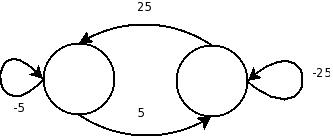
\includegraphics[height=2in,width=4in]{images/the_network_in_question_simple.jpeg}
\caption{Diagram showing the arrangement and weighted connection of neurons in the network from section 4.2.}
\end{center}
\end{figure}
\begin{figure}[htb]
\begin{center}
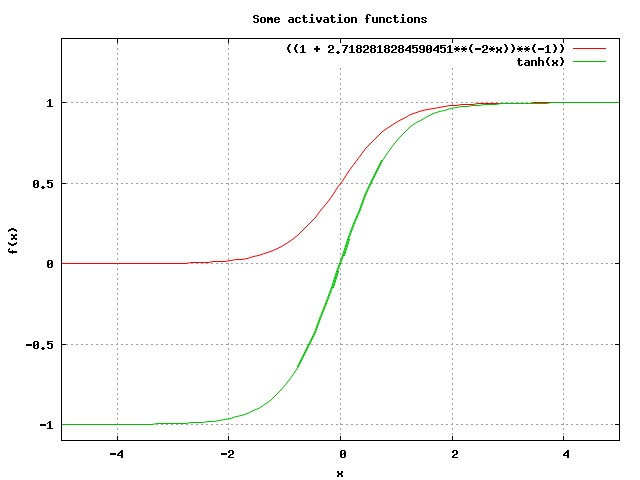
\includegraphics[height=2.5in,width=4.5in]{images/activation_funcs.jpg}
\caption{Two example activation functions.  One, the hyperbolic tangent.  Two, the sigmoidal function parameterized by $\mu$ used in the network from section 4.2}
\end{center}
\end{figure}

\begin{figure}[htb]
\begin{center}
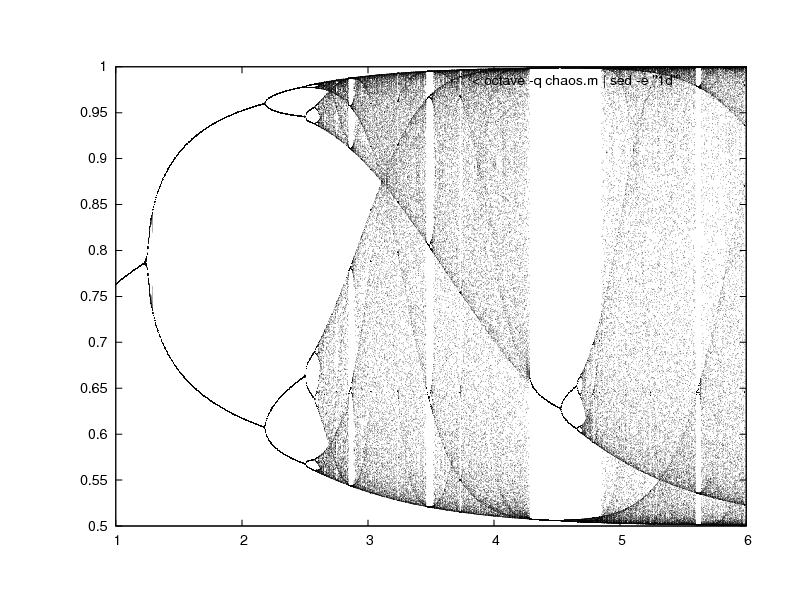
\includegraphics[height=2.5in,width=4.5in]{images/network_bifurc.png}
\caption{Bifurcation diagram of the network discussed in \cite{sole} and used as the system to be controlled in the proposal's preliminary experiments.  The horizontal axis is the parameter $\mu$ and the vertical axis is an approximation of one of the neurons' values along the system's attractor.  $\mu$ was held at $5.5$.}
\end{center}
\end{figure}
\begin{figure}[htb]
\begin{center}
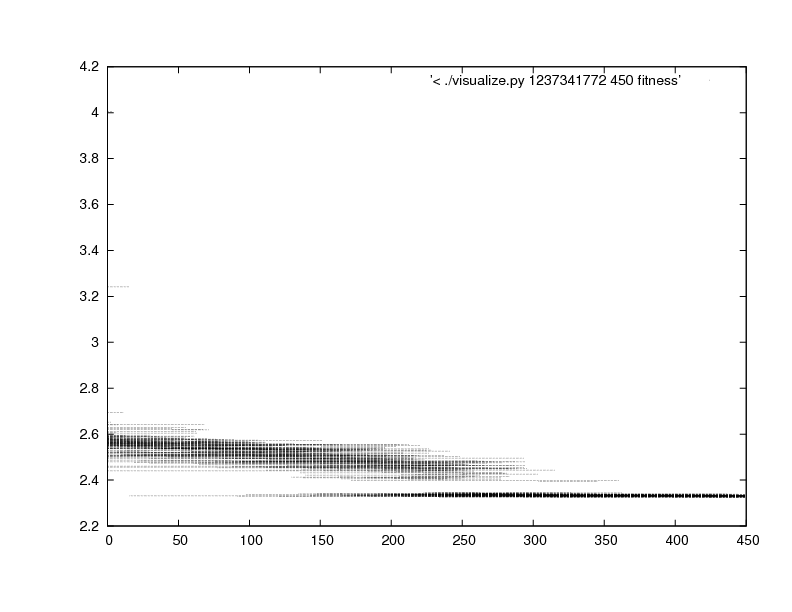
\includegraphics[height=2.5in,width=4.5in]{images/early_exp_greedy.png}
\caption{Evolutionary diagram of an early experiment with greedy selection and a binary alphabet for input sequence candidates.  The population converges early to an unacceptable solution.  Ticks on the horizontal axis are generations of the population and ticks on the vertical axis are fitness values (maximal Lyapunov exponents).}
\end{center}
\end{figure}
\begin{figure}[htb]
\begin{center}
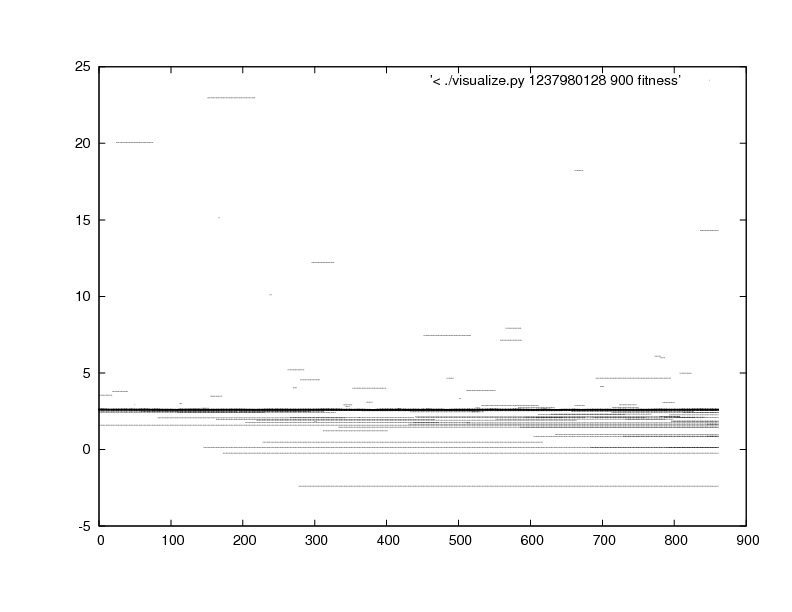
\includegraphics[height=2.5in,width=4.5in]{images/early_exp_non_greedy.png}
\caption{Evolutionary diagram of another early experiment with non-greedy selection and a binary alphabet for input sequence candidates.  What appears to be an acceptable sequence is found early on but the population doesn't converge to it.}
\end{center}
\end{figure}
\begin{figure}[htb]
\begin{center}
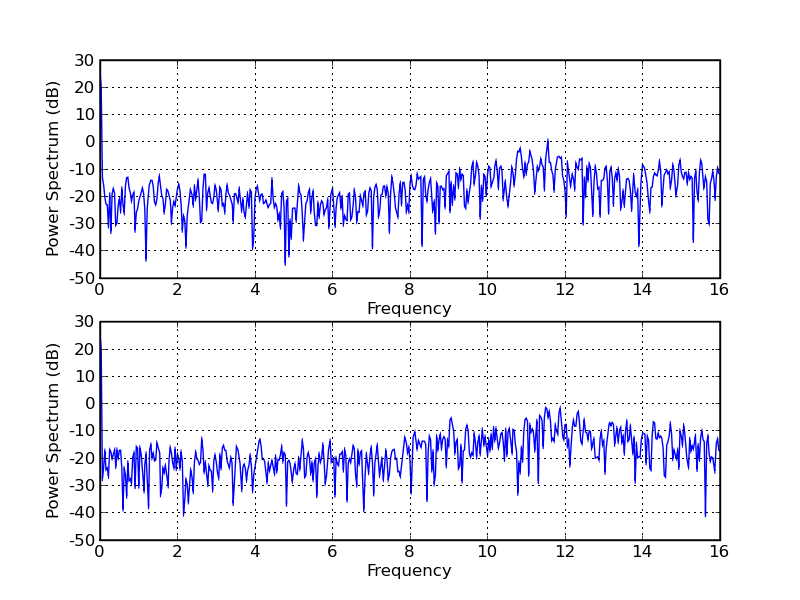
\includegraphics[height=2.5in,width=4.5in]{images/big_run_psd_small_amp.png}
\caption{Comparison of the power spectral density functions (PSD) of the
network with (above) and without (below) the 'hero' sequence of experiment 2.  Neither have distinguished peaks of periodicity and both indicate chaotic behavior, invalidating experiment 2.}
\end{center}
\end{figure}
\begin{figure}[htb]
\begin{center}
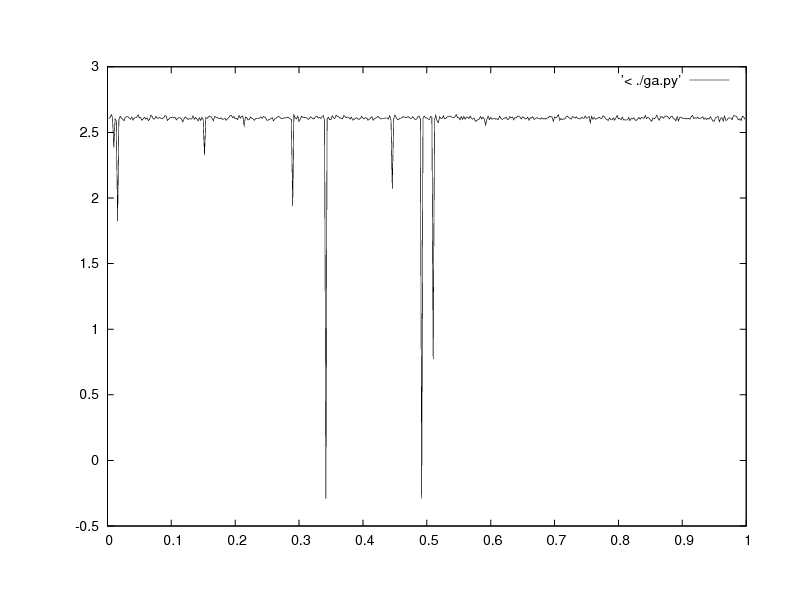
\includegraphics[height=2.5in,width=4.5in]{images/lyap_hero.png}
\caption{Lyapunov exponents of the network under perturbation by the hero sequence of experiment 2 but with varying initial seeds.  Horizontal axis is the chosen initial seed and vertical axis is the maximal Lyapunov exponent.  In the original run of the genetic algorithm, the seed was set to 0.34.}
\end{center}
\end{figure}
\begin{figure}[htb]
\begin{center}
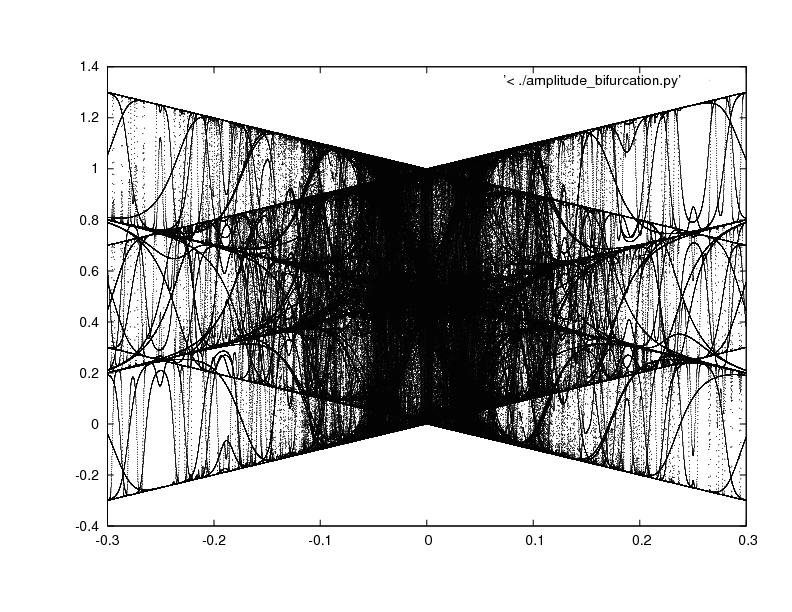
\includegraphics[height=2.5in,width=4.5in]{images/big_bifurcation.png}
\caption{Bifurcation diagram of the network under the influence of the hero from experiment 2 where $\alpha$ is allowed to vary from -0.3 to 0.3.  $\alpha$ is represented on the horizontal axis while the vertical axis is the approximate attractor for one of the neurons.}
\end{center}
\end{figure}

\begin{figure}[htb]
\begin{center}
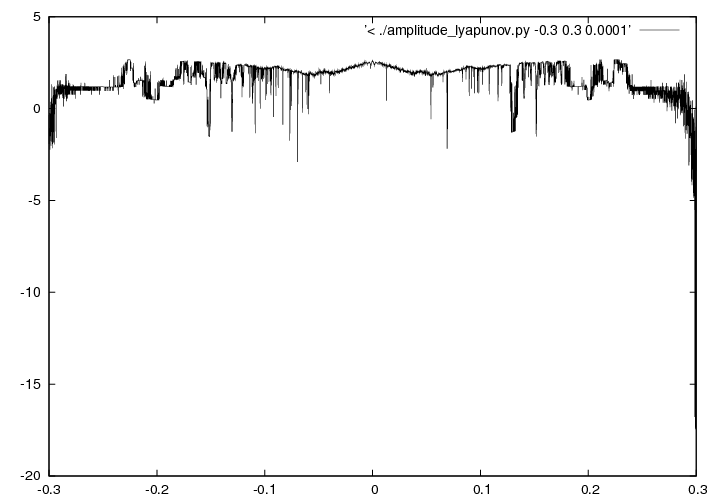
\includegraphics[height=2.5in,width=4.5in]{images/big_lyapunov.png}
\caption{Lyapunov exponents of the network under perturbation by the hero sequence of experiment 2 but with varying $\alpha$.}
\end{center}
\end{figure}



\begin{figure}[htb]
\begin{center}
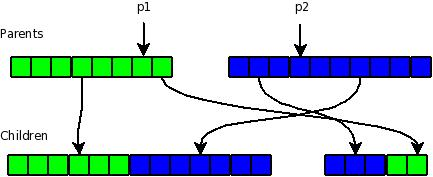
\includegraphics[height=2.5in,width=4.5in]{images/single_point_crossover.jpeg}
\caption{Random single point crossover.
    Subsequences of each parent sequence are selected by a random midpoint and exchanged to constitute complementary children.
}
\end{center}
\end{figure}

\begin{figure}[htb]
\begin{center}
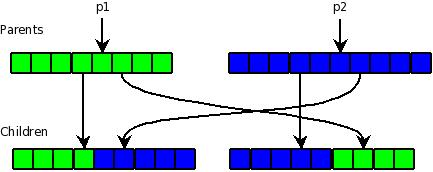
\includegraphics[height=2.5in,width=4.5in]{images/fixed_point_crossover.jpeg}
\caption{Fixed single point crossover.  Subsequences of each parent sequence are selected by a fixed midpoint and exchanged to constitute complementary children.}
\end{center}
\end{figure}

\begin{figure}[htb]
\begin{center}
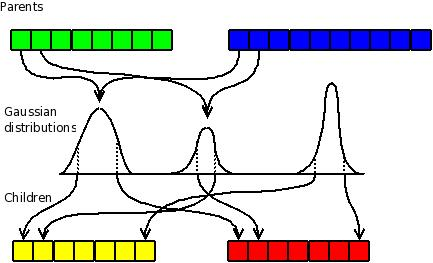
\includegraphics[height=2.5in,width=4.5in]{images/gaussian_crossover.jpeg}
\caption{
    Gaussian merge crossover.  The value of each element of two parents are taken as standard deviations from a mean and used to construct a Gaussian distribution.  A random value is drawn from the distribution.  Its value is used as the value of the corresponding element in the first child's sequence and its complimentary value is used for the second child.
}
\end{center}
\end{figure}

\begin{figure}[htb]
\begin{center}
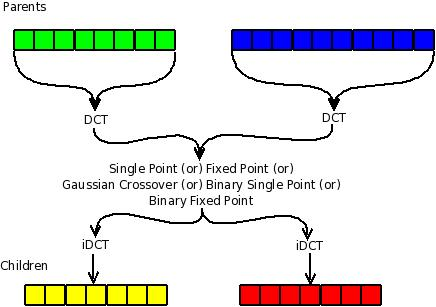
\includegraphics[height=2.5in,width=4.5in]{images/dct_crossover.jpeg}
\caption{
    Discrete Cosine Transform operators.  This concept is applied to all previously described crossover operators.  Input sequences are transformed to the frequency domain, crossover is performed and the produced children are then inverted back into the phase domain.
}
\end{center}
\end{figure}

\begin{figure}[htb]
\begin{center}
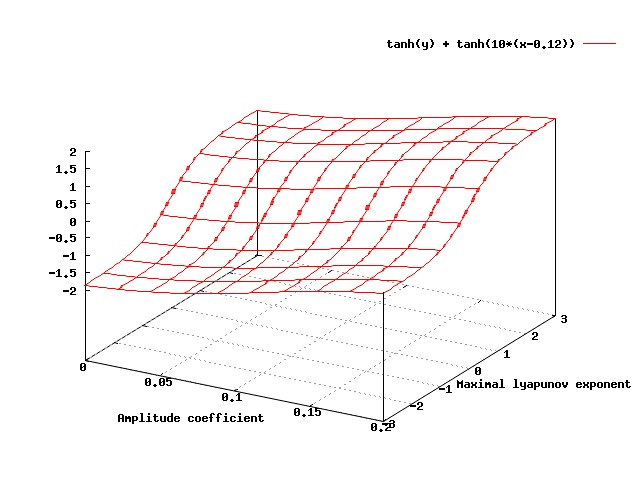
\includegraphics[height=2.5in,width=4.5in]{images/fitness_surface3.jpg}
\caption{ Surface of the "Tanh Combination Metric" fitness function where y represents the maximal Lyapunov number and x represents $\alpha$}
\end{center}
\end{figure}
\begin{figure}[htb]
\begin{center}
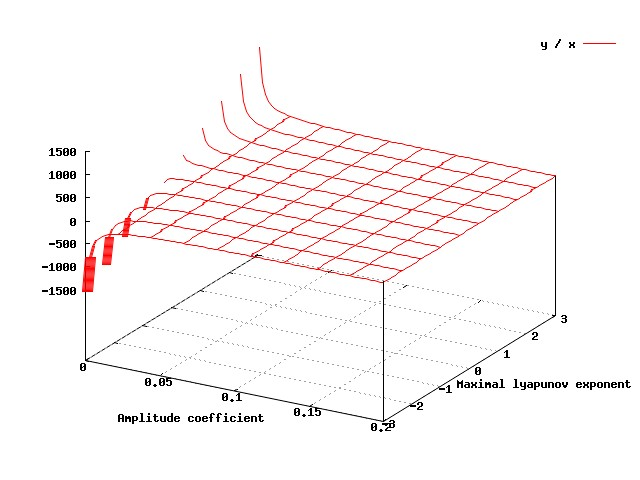
\includegraphics[height=2.5in,width=4.5in]{images/fitness_surface2.jpg}
\caption{ Surface of the "Division Metric" fitness function where y represents the maximal Lyapunov number and x represents $\alpha$}
\end{center}
\end{figure}
\begin{figure}[htb]
\begin{center}
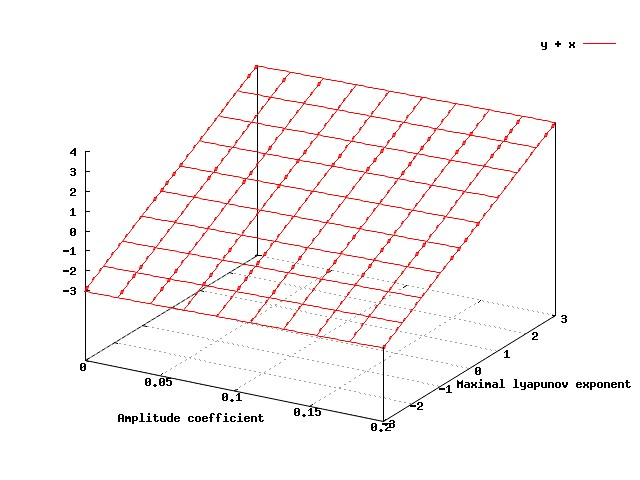
\includegraphics[height=2.5in,width=4.5in]{images/fitness_surface1.jpg}
\caption{ Surface of the "Addition Metric" fitness function where y represents the maximal Lyapunov number and x represents $\alpha$}
\end{center}
\end{figure}
\clearpage

\begin{figure}[htb]
\begin{center}
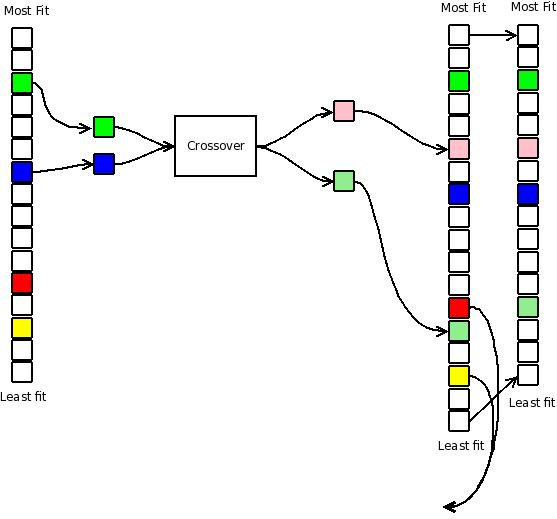
\includegraphics[height=2.5in,width=4.0in]{images/non_greedy_selection.jpeg}
\caption{Illustration of the non greedy selection method.}
\end{center}
\end{figure}
\begin{figure}[htb]
\begin{center}
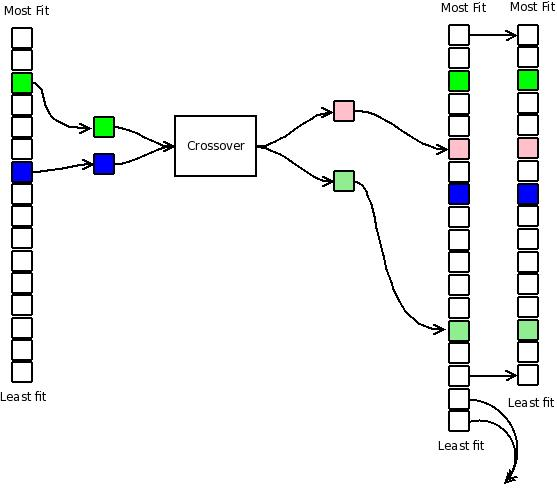
\includegraphics[height=2.5in,width=4.0in]{images/greedy_selection.jpeg}
\caption{Illustration of the greedy selection method.}
\end{center}
\end{figure}

\begin{figure}[htb]
\begin{center}
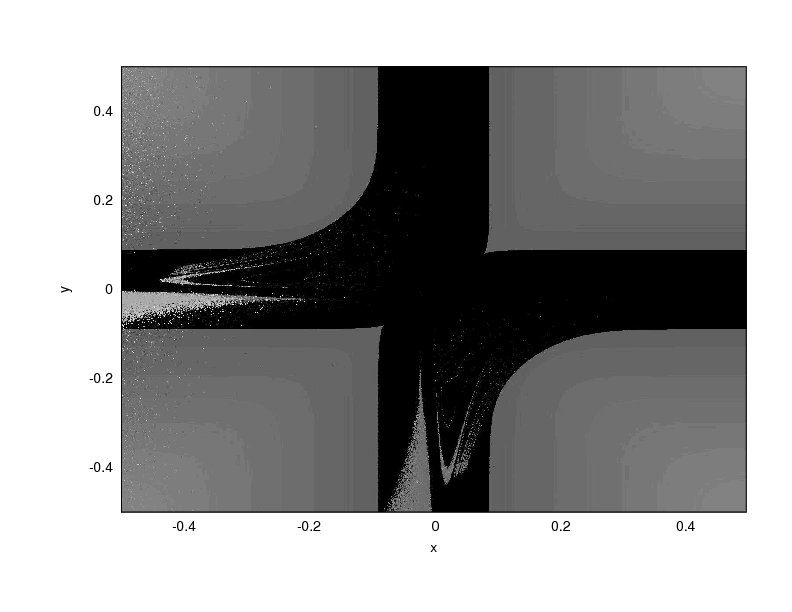
\includegraphics[height=4in,width=6.0in]{images/sample1.pdf}
\caption{Fitness map for the toy class of period-2 solutions shown from $x\in[-0.5:0.5], y\in[-0.5:0.5]$}
\end{center}
\end{figure}
\begin{figure}[htb]
\begin{center}
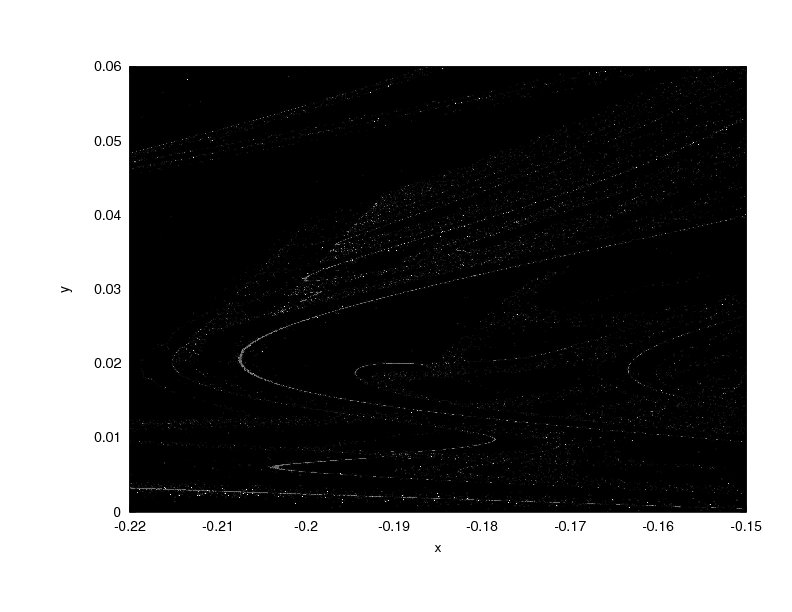
\includegraphics[height=4in,width=6.0in]{images/sample2.pdf}
\caption{A subset of figure 20 enlarged to show detail at $x\in[-0.22:-0.15], y\in[0:0.06]$}
\end{center}
\end{figure}
\begin{figure}[htb]
\begin{center}
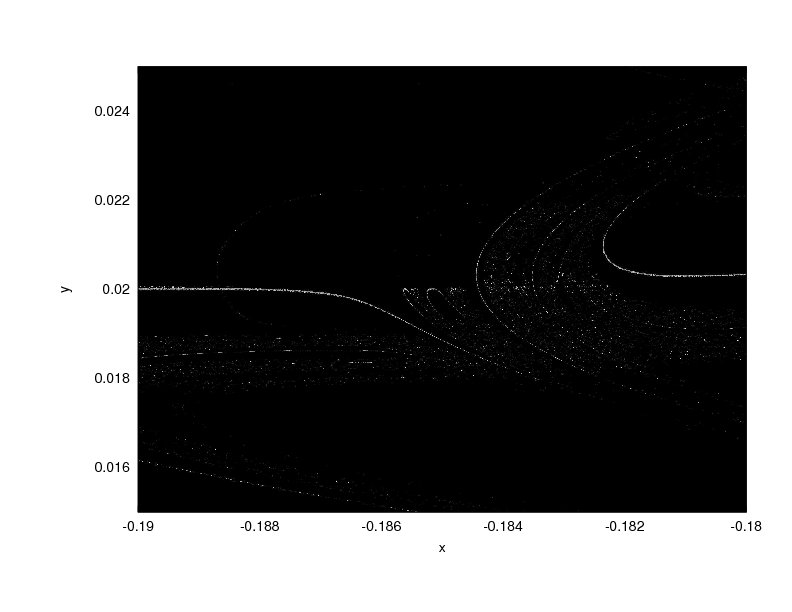
\includegraphics[height=4in,width=6.0in]{images/sample3.pdf}
\caption{A subset of figure 21 enlarged to show detail at $x\in[-0.19:-0.18], y\in[0.015:0.025]$}
\end{center}
\end{figure}
\begin{figure}[htb]
\begin{center}
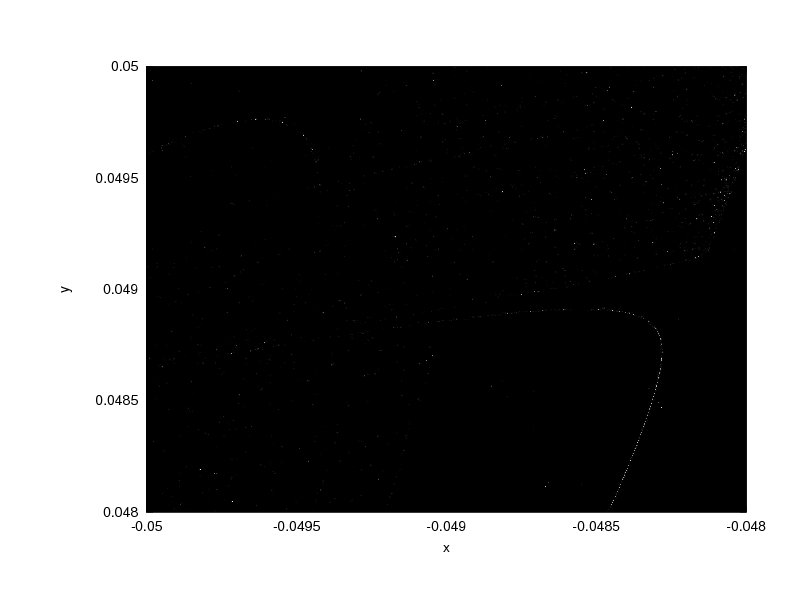
\includegraphics[height=4in,width=6.0in]{images/sample4.pdf}
\caption{Another subset of figure 20 enlarged to show detail.  Chosen to be close to the origin at $x\in[-0.05:-0.048], y\in[0.048:0.5]$}
\end{center}
\end{figure}

\end{document}

